\documentclass[11pt]{article}
%\documentclass{minimal}
\usepackage[annataritalic]{tengwarscript}
\usepackage[utf8]{inputenc}
\usepackage{graphicx}
\usepackage{url}
\usepackage{fancyhdr}
\usepackage{titling}
\usepackage{soul}
\usepackage{natbib}
\usepackage[top=1in,bottom=1in,left=1.5in,right=1.5in]{geometry}
%\usepackage{fullpage}
\title{AHP FOR STUDENT DECISIONS IN A MONTESSORI ELEMENTARY CLASS}
\pagestyle{fancy}
\chead{}
\lhead{\textit{ISAHP Article: \thetitle}}
\rhead{}
\lfoot{\textit{International Symposium on the \\ Analytic Hierarchy Process}}
\cfoot{\thepage}
\rfoot{London, U.K. \\ August 4-7, 2016}
\renewcommand{\headrulewidth}{0pt}
\renewcommand{\footrulewidth}{0pt}
\renewcommand{\maketitle}{\begin{center}{\Large \textbf{\thetitle}} \end{center}}
%%%Numbered bib section
\renewcommand{\bibsection}{\section{Key References}}
%%%%%%%%%
\begin{document}
\maketitle
\thispagestyle{fancy}

\begin{abstract}
In this paper we devise and use a new pairwise comparison questionnaire based upon a
Liskert scale that enables
Montessori elementary students to express their preferences for classroom jobs and
areas of cleaning responsibility.  In addition we developed the SimpleAHP web application
so that elementary students could analyze the results of their questionnaires on their
own.  We find that the simplified questionnaire worked well with our students and holds
promise to allow more people access to AHP.


%A Montessori elementary class consists of students aged 6-12.  Part of the Montessori educational
%process is giving the students responsibilities and decisions to make for their class.
%In this paper we use a simplified scale for pairwise comparisons to find indvidual preferences
%for classroom duties.  In addition we developed a web application, SimpleAHP, that performs the 
%standard largest eigenvector calculations using this scale, or the traditional 1-9 scale.
%We use SimpleAHP to analyze individual, group, and demographic subgroup preferences for our
%particular problem.  We find that the simplified scale works very well for untrained and/or
%young participants, and that SimpleAHP is quite usable for young facilitators to find insights
%and preferences of participants, the overall group and demographic subgroups.
\end{abstract}


\section{Introduction}
Maria Montessori developed a teaching method in the early 1900's that is still popular today, called the Montessori method.  Schools that follow this method are called Montessori schools.  For more information about the Montessori method, see \citep{montessori2013montessori}.  Part of that method is students are responsible for maintaining their classroom, and in our class students are assigned areas of the classroom to clean, and jobs in those areas.

If we know students preferences for jobs and areas, we could
try to assign them jobs they enjoy in areas they prefer, which could
make them happier and more productive.  We use a pairwise comparison
process to accomplish this goal.  A difficulty in this approach is
the traditional 1-9 scale is hard to understand, especially for students
aged 6-12.  We decided to simplify the standard scale to a Likert type
scale we call the \ul{EBM scale} (meaning \emph{Equals}, 
\emph{Better}, and \emph{Much Better}) and develop the \ul{SimpleAHP}
web application to perform the calculations and present the analysis in a
way that students could navigate and understand.  This research could help our class
better handle job assignments, and the EBM scale approach and SimpleAHP web
application could make AHP
easier for anyone to understand.


\section{Literature Review}
It is difficult to find references for teaching youths to use AHP for
decision making.  In the paper \citep{ref1} the authors explore
using AHP in a higher educational setting, not a primary education setting.
There were no tools available to help youth frame useful questions, solicit
preference data, and analyze their results.  
We used the EBM scale, which is a Likert scale with 5 items, based upon
the research in \citep{matell1971there} for our simplified questionnaire format.
We also created the SimpleAHP web application as a tool that youth
could use to analyze their data, using the Shiny \citep{shiny} web toolkit
for the R \citep{R} programming language.

\section{Hypotheses/Objectives}
Our research has three objectives: first to figure out the job and area
preferences for our class, second to simplify the pairwise 
questionnaire process for ease of use for young students (although
the simplification could be used by anyone), and third to create a tool students
could use to analyze this simplified preference data.


%Your study may be trying to prove something or at the very least will have a specific objective (e.g. development of a decision model for a particular problem). Make sure to list them here. The reader must be clear about the specific objectives or hypotheses in your study. 

\section{Research Design/Methodology}
We decided to do a single goal AHP model, i.e. one pairwise comparison set,
for the areas and another pairwise comparison set for the jobs.  We did this, in part, because
leading 6-12 year olds through a complete comparison set for a full AHP model would be
difficult.  In addition, we wanted to create a process other students could follow to
solve their own problems.   A complex AHP/ANP model would be difficult for younger participants
as well as those new to AHP/ANP.

We created a new questionnaire format using the EBM scale (see Figure \ref{fig:2}
for an example), and
decided upon default values for those votes of 1, 4.5, and 9 respectively.  We decided 
on the these numerical values for two reasons, first it breaks up the 1-9 scale into two equal
segments, and secondly for our data it provided for good differentiation.  Additionally we
designed the SimpleAHP web application that allows for the use of the EBM scale and
allows one to change their numerical values.

%This is an important part of a study. If you are developing an AHP/ANP model, it is important to explain how the model came to be. Typically, a model is based on information of secondary sources (literature review), pool of experts, user surveys, or a combination of sources. It is important that you explain how goal, criteria, alternatives, influences and judgments were obtained. In particular, if the opinion of different people were aggregated, explain how this aggregation took place. Similarly, indicate how you addressed inconsistency problems. Otherwise your proposed model will have a bad start for lack of face validity.

\section{Data/Model Analysis}
Our model for the jobs as well as the areas decision was a simple pairwise comparison
amongst the alternatives.  The overall results by gender can be seen in Figure \ref{fig1}
and further results are available through the SimpleAHP web application
at \url{http://tiny.cc/youthAHPOut1} for the areas and
\url{http://tiny.cc/youthAHPOut2} for the jobs.

There was an interesting piece of work needed to reduce the number of job choices.
The class actually has approximately 20 distinct jobs across the areas.  Pairwise
comparing 20 jobs is far too much for anyone to do.  Therefore we searched for
commonality across jobs to group like jobs together.  After much work and discussion
we were able to identify 5 job types, and that is what we used for the jobs
choice question.  We needed to make sure the job names indicated, intuitively, the
meaning of the work being done, so that students would understand the pairwise
comparison choices presented to them.
\begin{figure}
\caption{Results by Gender}
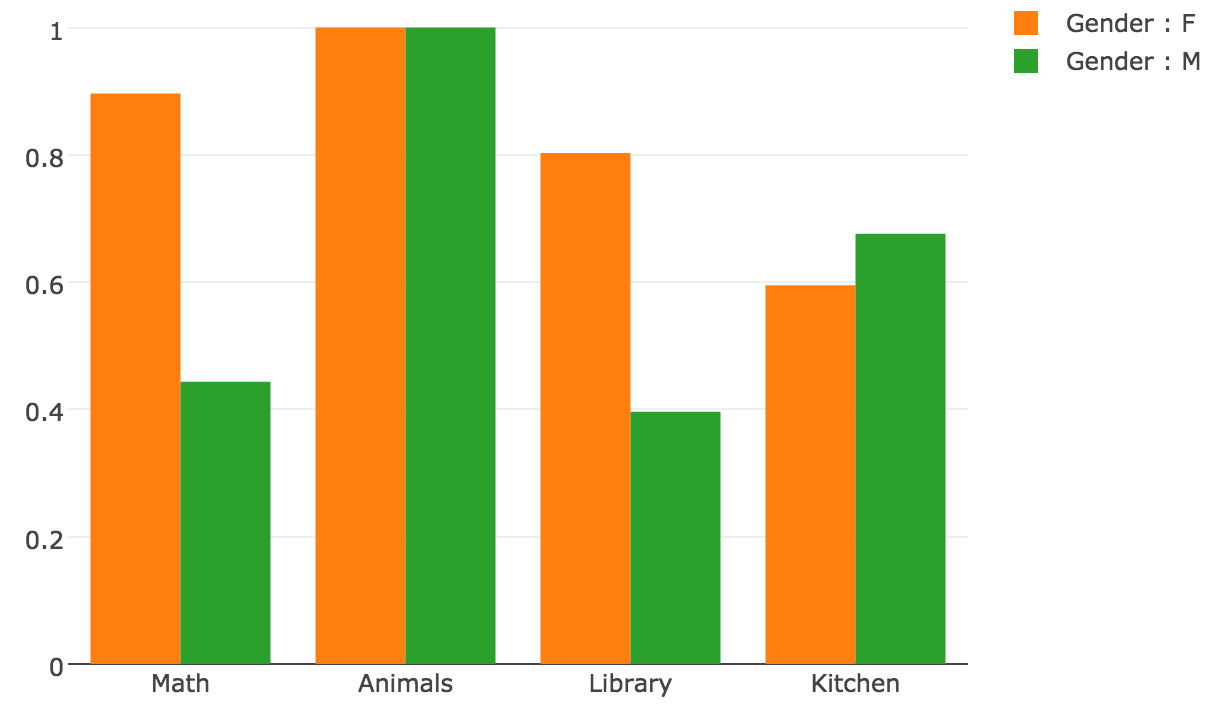
\includegraphics[width=2.5in]{AreasByGender}
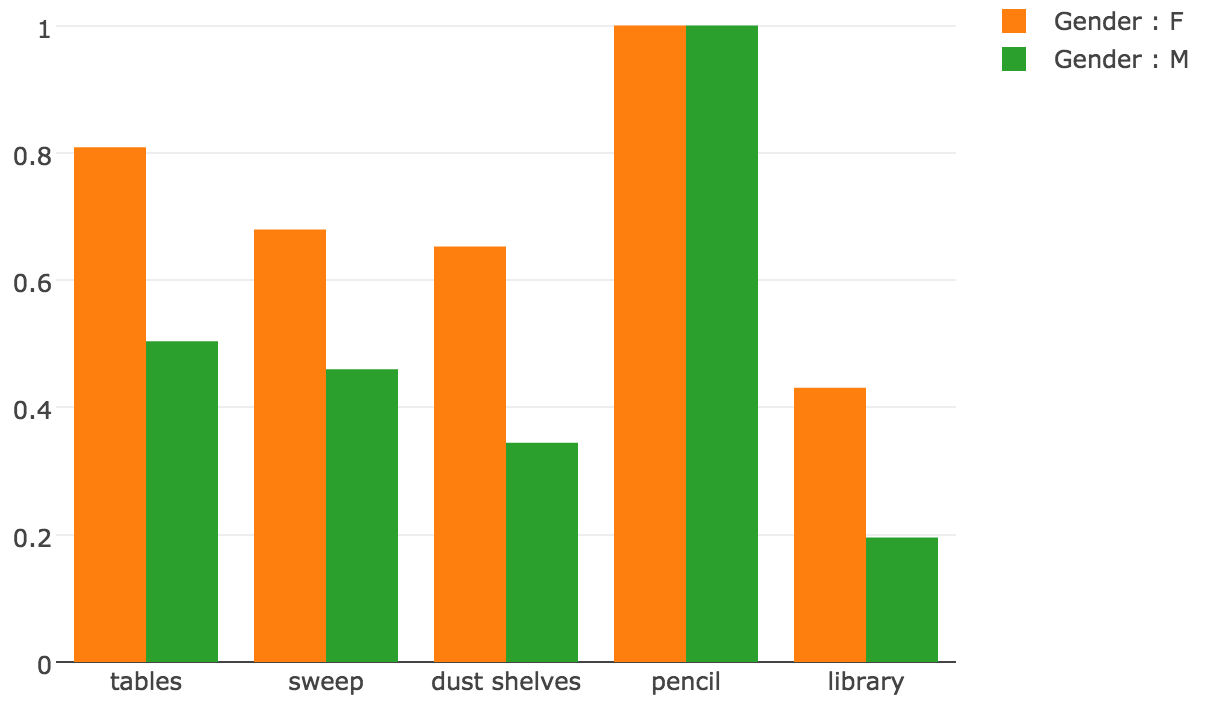
\includegraphics[width=2.5in]{JobsByGender}
\label{fig1}	
\end{figure}

%If you are developing an AHP/ANP model, make sure to show the hierarchy or network respectively. Show the judgment matrices or if the model is too big, show sample matrices. Make sure to provide the key indicators (e.g. consistency indices) to ensure your model is valid. Use the graphic to include additional information such as local weights, C.I., etc. Remember the old saying that a good drawing is worth 10,000 words!

\section{Limitations}
In our particular models for jobs and areas, our pairwise votes are on the EBM scale, which is not as precise as the standard 1-9 scale.  On the other hand, the standard 1-9 scale would have been more complicated than it should have been, especially for untrained students to participate in.
(Our SimpleAHP application can accept votes either in the 1-9 scale or the Better, Much Better scale equally easily, so that limitation is not a problem for our application.)

In addition, we did not attempt to do either a full AHP or ANP model with
the students.  We felt this was necessary for two reasons.  First, we did not
want the students to get bogged down in too many pairwise comparisons.  Second, we
wanted to create a reproducible process that other students could follow.  We were
able to easily state our problems in this fashion, but other student decisions may
not be amenable to this infrastructure.
%Given the reality of our physical world, no study is perfect. Please, indicate which are those aspects of the study you could not solve satisfactorily and that could weaken the value of your model. What you would different should you have the opportunity to start over? These considerations are important to assess the context of your model validity and also as a way to mentor colleagues interested in this stream of scholarship. 

\section{Conclusions}
The EBM scale, combined with the simplified questionnaire 
shown in Figure \ref{fig:2},
allowed our young voters to easily participate and understand both the 
questions and the
problems.  The SimpleAHP web application allowed us to analyze our findings overall, by
individuals and by groups easily.  In addition our process shows promise
to be useful for
other people who want to answer similar questions, without the need to 
understand all of the
technical details of AHP/ANP theory.
%Now you have the opportunity to share with the world your contributions. What can you conclude from this study? What are your theoretical and/or practical contributions? How can you be certain of your achievements (e.g. is the model being used?) What are the next studies you would propose in this line of scholarship? How does your contribution fit or differs into (or from) the current stream of scholarship. Make sure that your conclusions are based on the current study and that clearly show an important contribution to the theory and/or practice of AHP/ANP. 


\bibliographystyle{apalike}
\bibliography{OurPapers}

 \section{Appendix 1}
%\begin{center}
%	Just a closing thought:
%\end{center} 
 
\begin{minipage}[t]{0.5\textwidth}
 \tengwarannataritalic[1.09]
 \tengwa{254}
 \Textendedcalma\TTthreedots\Tnuumen\Tessenuquerna\TTthreedots\Tungwe\Tando\Toore\TTrightcurl\Tumbar\Ttinco\TTthreedots\Tlambealt\TTrightcurl\Tquesse\TTdoublerightcurl
 \Tromanperiod\Ts
 \Textendedcalma\TTthreedots\Tnuumen\Tessenuquerna\TTthreedots\Tungwe\Tungwe\Tumbar\TTnasalizer\TTdot\Ttinco\TTthreedots\Tlambe\TTrightcurl
 \tengwa{255}\\
 \Textendedcalma\TTthreedots\Tnuumen\Tessenuquerna\TTthreedots\Tungwe\Tthuule\Troomen\Tquesse\TTthreedots\Ttinco\TTthreedots\Tlambealt\TTrightcurl\Tquesse\TTdoublerightcurl
 \Tromanperiod\Ts
 \Textendedungwe\TTthreedots\Tumbar\Toore\TTrightcurl\Tesse\Tkern{-0.2}\Tmalta\TTrightcurl\Textendedcalma\TTdot\Ttelco\TTdot\Tquesse\Troomen\Tparma\TTnasalizer\TTdot\Ttinco\TTthreedots\Tlambe\TTrightcurl
 \newline
\end{minipage}
\begin{minipage}[t]{0.5\textwidth}
 One ring to rule them all \newline
 One ring to find them \newline
 One ring to bring them all \newline
 And in the darkness bind them
\end{minipage}

%{\telcontar 
%Ash nazg durbatulûk\newline
%ash nazg gimbatul\newline 
%ash nazg thrakatulûk \newline 
%agh burzum-ishi krimpatul
%}

\section{Appendix 2}
\begin{figure}[!hb]
\caption{Actual Questionnaire Students Filled Out For Areas Decision}
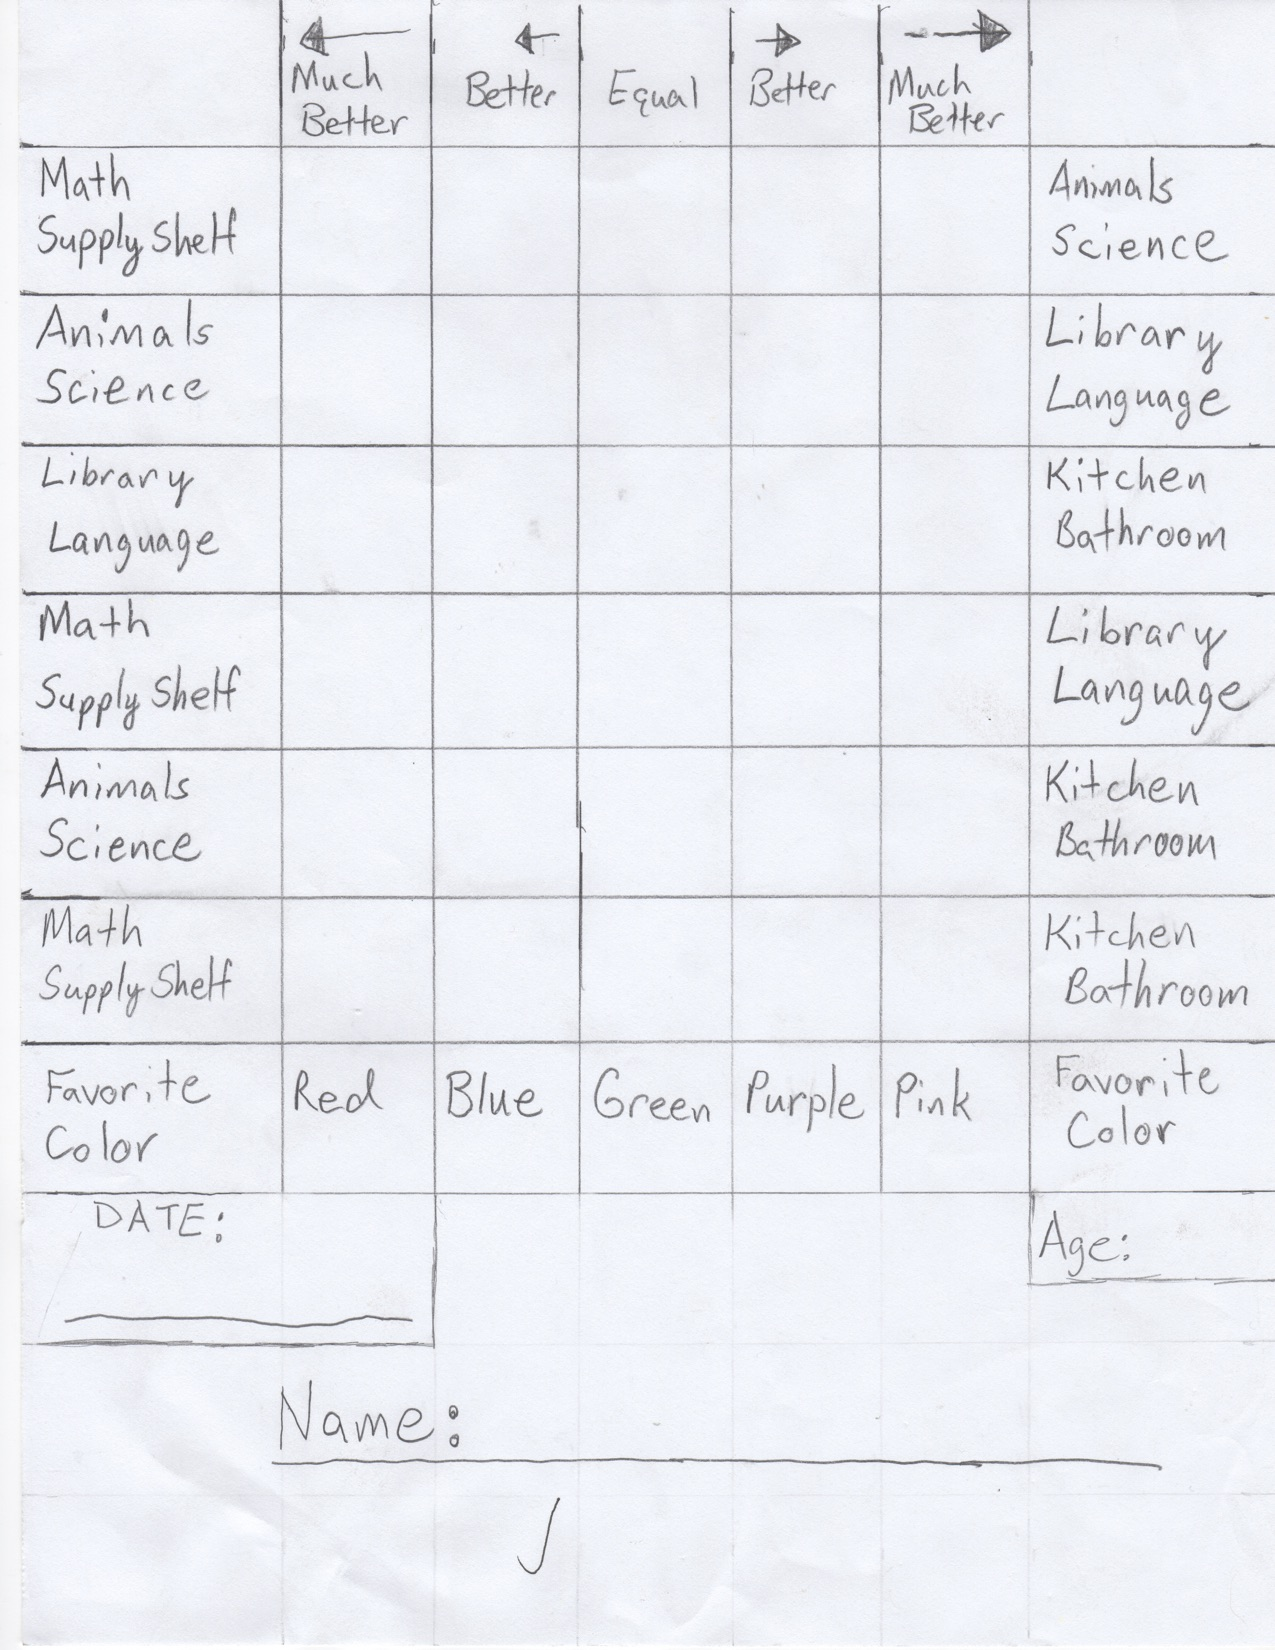
\includegraphics[height=5in]{SampleAHPQuestionnaire}
\label{fig:2}
\end{figure}


\end{document}